% fig1-cost-split.tex — §7 cost-split visualisation (RC-07)
% Data source: data/aggregated/cost-split.csv
% cost-split.csv columns: bucket,cost_usd,n_calls,cost_share_pct
%   session_total  115.54  500  100.0
%   main_thread    114.81  445  99.37
%   subagent_dispatch 0.7338 55 0.635
% Style: print-safe stacked bar (horizontal), width=0.85\textwidth

\begin{figure}[ht]
\centering
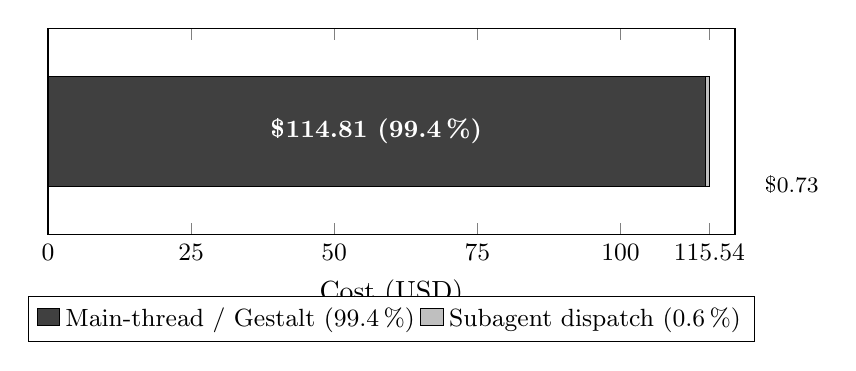
\begin{tikzpicture}
\begin{axis}[
  xbar stacked,
  width=0.85\textwidth,
  height=4.2cm,
  bar width=1.4cm,
  xmin=0, xmax=120,
  ymin=-0.5, ymax=0.5,
  ytick=\empty,
  xlabel={Cost (USD)},
  xtick={0,25,50,75,100,115.54},
  xticklabel style={font=\small},
  legend style={
    at={(0.5,-0.30)},
    anchor=north,
    legend columns=2,
    font=\small,
    draw=black,
  },
]
% Main-thread bar (99.4%)
\addplot+[
  fill=black!75,
  draw=black,
  nodes near coords={\$114.81 (99.4\,\%)},
  nodes near coords align={center},
  every node near coord/.append style={font=\small\bfseries, color=white},
] coordinates {(114.81, 0)};

% Subagent dispatch bar (0.6%)
\addplot+[
  fill=black!25,
  draw=black,
] coordinates {(0.7338, 0)};

\legend{Main-thread / Gestalt (99.4\,\%), Subagent dispatch (0.6\,\%)}
\end{axis}
% Annotation for the thin subagent bar
\node[anchor=west, font=\footnotesize] at (current bounding box.east)
  {\$0.73};
\end{tikzpicture}

\caption{%
  Single-window cost split (\$115.54 over 7 days, \texttt{claude-opus-4-7});
  main-thread dominates by two orders of magnitude, motivating per-turn
  routing as the primary cost lever.
  Source: \texttt{data/aggregated/cost-split.csv}.%
}
\label{fig:cost-split}
\end{figure}
